%note: don't split this document up with include{...}

\section{CodeProcessor}

\subsection{Klassendiagramm}

\begin{figure}[htbp] 
  \centering
  		 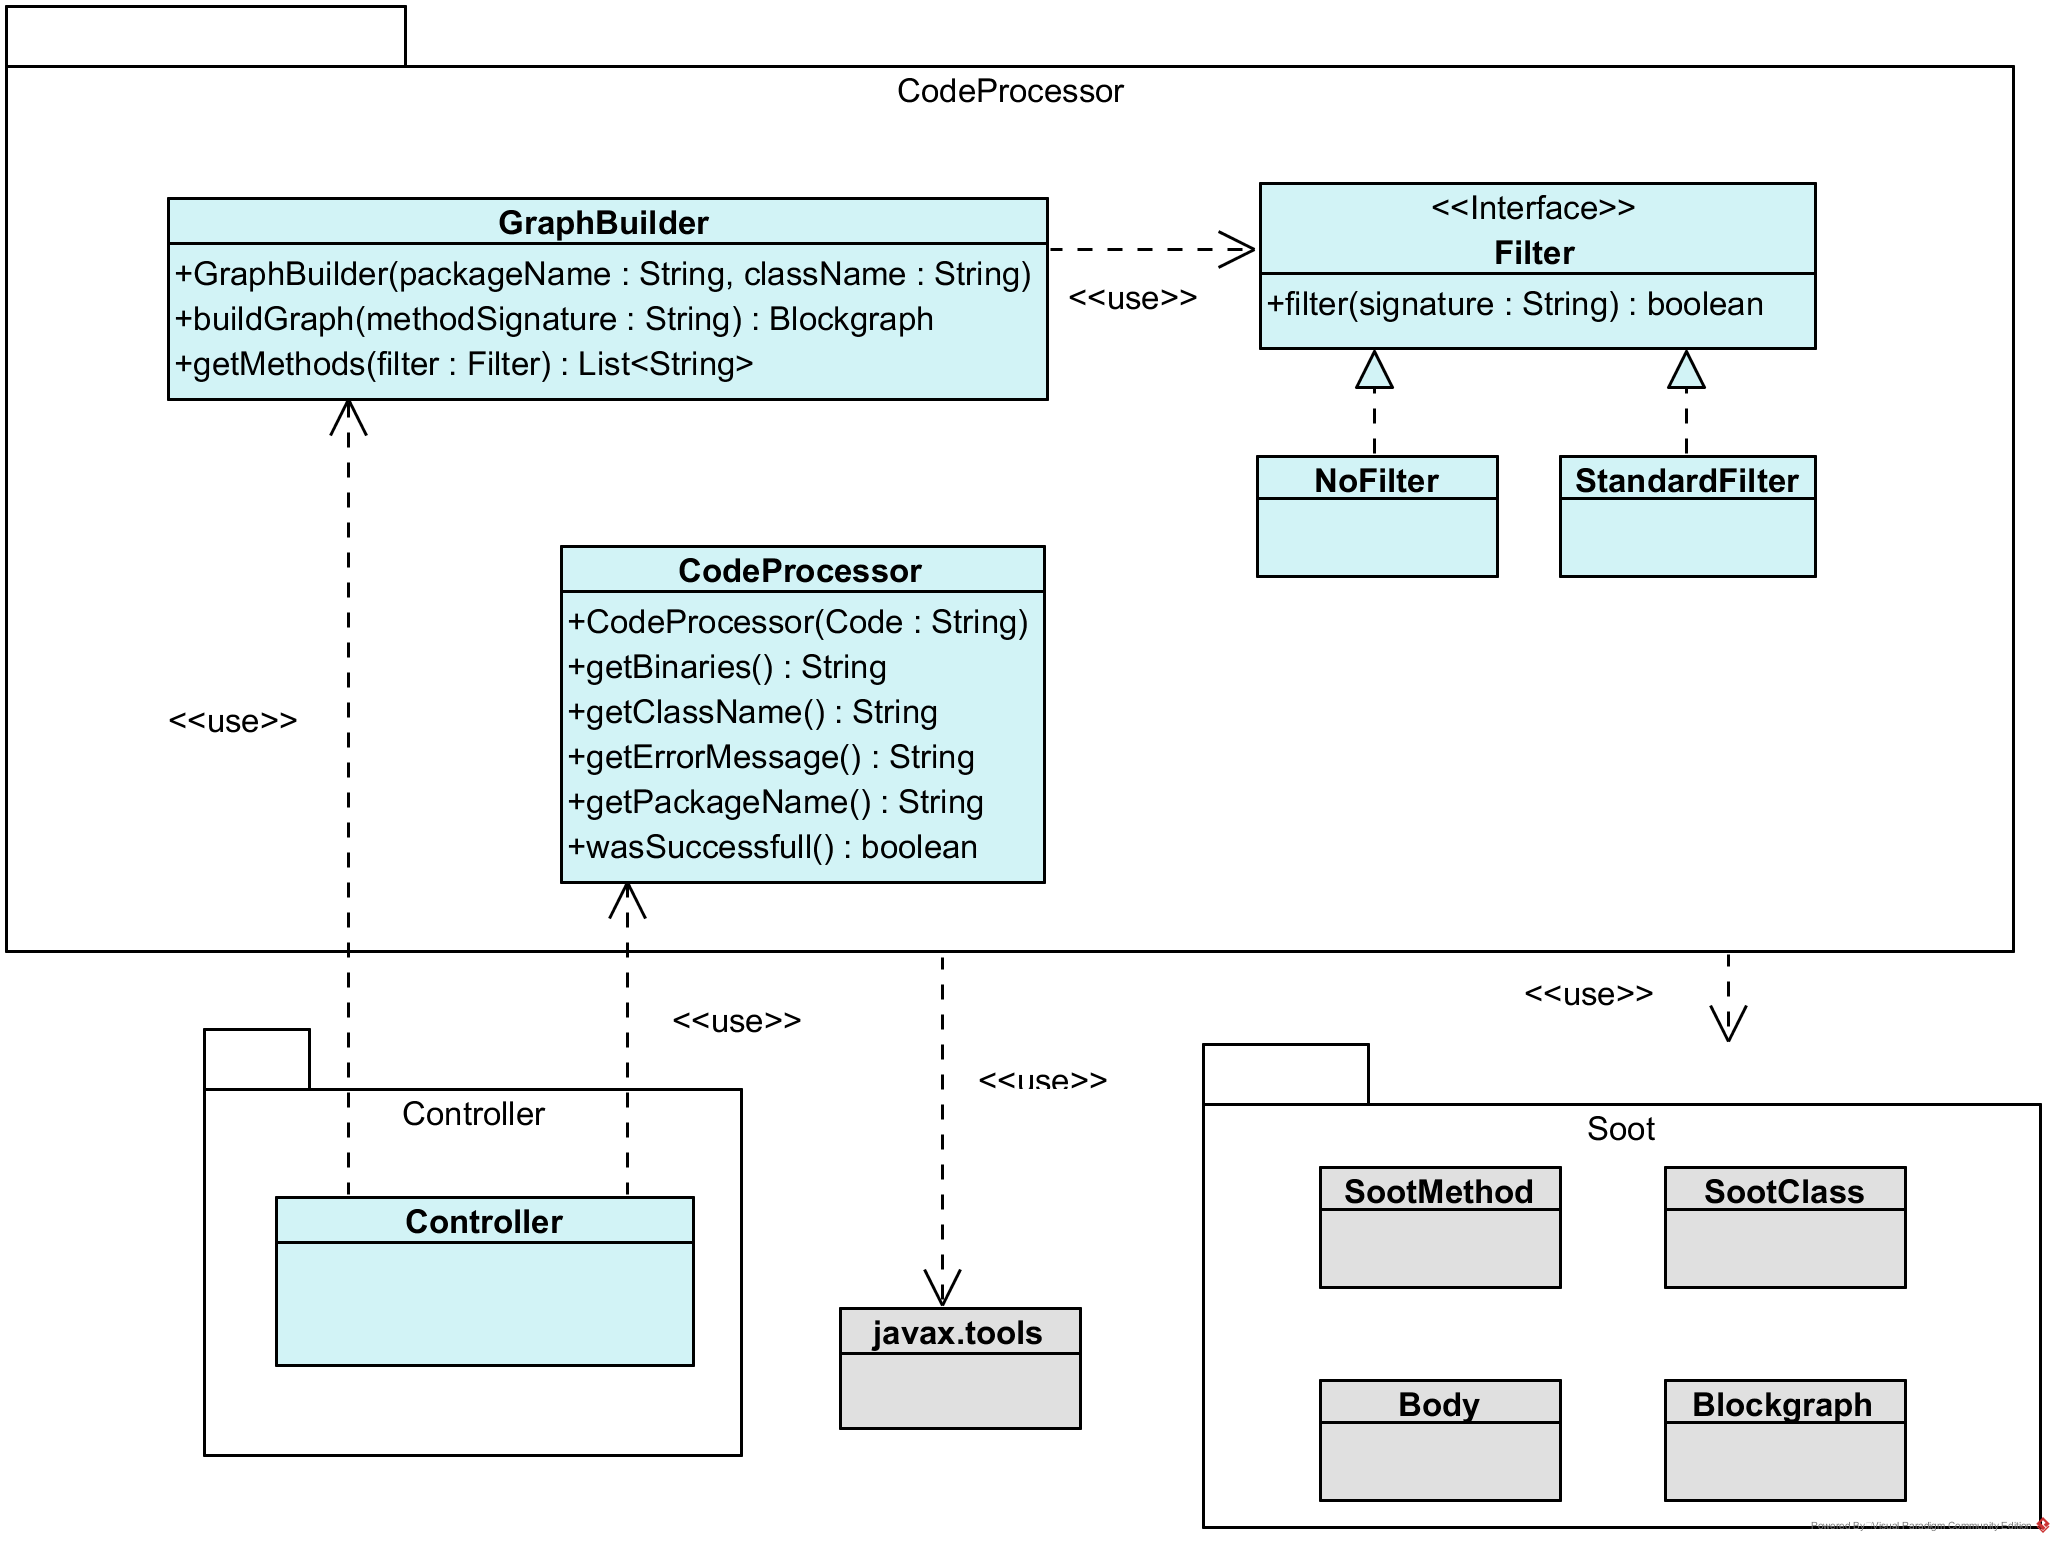
\includegraphics[width=1\textwidth]{Klassenuebersicht/CodeProcessor/CodeProcessor}
  \caption{Klassendiagramm des User Interfaces}
  \label{fig:UI}
\end{figure}

\subsection{Modulbeschreibung}

Das CodeProcessor-Modul ist dafür verantwortlich den eingegebenen Code des Benutzers in Java-Bytecode und letztendlich in einen Kontrollflussgraphen umzuwandeln, welcher in der weiteren Programmlogik verwendet werden kann.

Es gibt zwei Schnittstellen; \inlinecode{CodeProcessor} und \inlinecode{GraphBuilder}.
Der \inlinecode{CodeProcessor} erhält vom \inlinecode{Controller} den eingegebenen Code des Benutzers und versucht diesen zu Java-Bytecode zu kompilieren.

Ist dies erfolgreich, so ruft der \inlinecode{Controller} den \inlinecode{GraphBuilder} auf und lässt den Java-Bytecode mithilfe der externen Bibliothek Soot in eine Zwischenrepräsentation umwandeln.
Aus dieser können dann alle Methoden ausgelesen werden, welche in dem zu analysierenden Code enthalten sind.
Aus diesen Methoden können über das Interface \inlinecode{Filter}, beziehungsweise seine Implementierungen uninteressante Methoden, wie zum Beispiel geerbte Methoden herausgefiltert werden.
Abschließend kann man dem \inlinecode{GraphBuilder} die Signatur der zu analysierenden Methode übergeben und erhält einen \inlinecode{BlockGraph} zu der entsprechenden Methode, welcher in der weiteren Programmlogik verwendet werden kann.

\subsection{Klassenbeschreibung}

\class{CodeProcessor}
%Brief descrition of SomeClass.
Verarbeitet den vom Benutzer eingegebenen Java-Sourcecode zu Java-Bytecode.

\subparagraph{Konstruktoren} % skip this if there are no constructors
\begin{itemize}
	\item \ctor{CodeProcessor}{code : String}{public}{
		Überprüft ob der gegebene Code eine Klasse ist, welche Methoden beinhaltet und fügt die gegebenenfalls benötigten Strukturen hinzu. Der Code wird dann zu Java-Bytecode kompiliert.
		Ist dies erfolgreich so kann der Benutzer den kompilierten Code über die restlichen Methoden der Klasse erhalten.
	}
\end{itemize}

\subparagraph{Methoden}  % skip this if there are no methods
\begin{itemize}
	\item \method{getClassName}{String}{}{public}{
		Gibt den Namen der kompilierten Klasse zurück, falls das Kompilieren erfolgreich war.
	}
\end{itemize}

\begin{itemize}
	\item \method{getPackageName}{String}{}{public}{
		Gibt den Namen des Paketes der kompilierten Klasse zurück, falls das Kompilieren erfolgreich war.
	}
\end{itemize}

\begin{itemize}
	\item \method{wasSuccessfull}{boolean}{}{public}{
		Gibt \inlinecode{true} zurück, wenn das Kompilieren erfolgreich war, \inlinecode{false} wenn nicht.
	}
\end{itemize}

\begin{itemize}
	\item \method{getErrorMessage}{String}{}{public}{
		Gibt eine Fehlerbeschreibung als \inlinecode{String} zurück, falls beim Kompilieren des Codes ein Fehler aufgetreten ist.
	}
\end{itemize}

\begin{itemize}
	\item \method{getBinaries}{String}{}{public}{
		Gibt den kompilierten Java-Bytecode als String zurück, falls das Kompilieren erfolgreich war.
	}
\end{itemize}

\class{GraphBuilder}
%Brief descrition of SomeClass.
Diese Klasse verarbeitet Java-Bytecode zu einem \inlinecode{BlockGraph}.


\subparagraph{Konstruktoren} % skip this if there are no constructors
\begin{itemize}
	\item \ctor{GraphBuilder}{packageName : String, className : String}{public}{
		Über den Klassennamen und den Paketnamen wird der Java-Bytecode mithilfe der Bibliothek Soot zu einer \inlinecode{SootClass} umgewandelt.
	}
\end{itemize}

\subparagraph{Methoden}  % skip this if there are no methods
\begin{itemize}
	\item \method{getMethods}{List<String>}{filter : Filter}{public}{
		Gibt eine Liste aller Methodensignaturen in der \inlinecode{SootClass} zurück, die nicht mithilfe des \inlinecode{Filters} ausgeschlossen wurden.
	}
\end{itemize}

\begin{itemize}
	\item \method{buildGraph}{BlockGraph}{methodSignature : String}{public}{
		Verarbeitet mit Hilfe der Bibliothek Soot eine Methode aus der \inlinecode{SootClass} zu einem \inlinecode{BlockGraph}.
		Dieser ist ein Kontrollflussgraph, welcher im weiteren Programm verwendet werden kann.
	}
\end{itemize}

\class{<<Interface>> Filter}
%Brief descrition of SomeClass.
Die Implementierungen dieses Interfaces können Methodensignaturen filtern, um somit zum Beispiel geerbte Methoden herauszufiltern.



\subparagraph{Methoden}  % skip this if there are no methods
\begin{itemize}
	\item \method{filter}{boolean}{MethodSignature}{public}{
		Gibt \inlinecode{true} zurück, falls die Methode herausgefiltert werden soll, \inlinecode{false} wenn nicht.
	}
\end{itemize}

\class{NoFilter implements Filter}
%Brief descrition of SomeClass.
Eine Implementierung eines \inlinecode{Filters}, welcher keine Klassen herausfiltert.

\class{StandardFilter implements Filter}
%Brief descrition of SomeClass.
Eine Implementierung eines \inlinecode{Filters}, welcher alle geerbten Methoden herausfiltert.